\documentclass{article}
\usepackage[utf8]{inputenc}
\usepackage{fancyhdr}
\usepackage{lastpage}
\usepackage{graphicx}
\usepackage{hyperref}
\usepackage{natbib}
\usepackage{amsmath,amstext}
\bibliographystyle{aasjournal}
\usepackage{pythonhighlight}
\usepackage{float}
\usepackage{listings}
\lstset{basicstyle=\ttfamily,
  showstringspaces=false,
  commentstyle=\color{red},
  keywordstyle=\color{blue}
}

\pagestyle{fancy}
\usepackage[margin=1in]{geometry}
\headwidth = 6.5in

\fancyhf{}
\headheight = 0.6in
\topmargin = -0.5in
\newcommand{\version}{v0.5}

\lhead{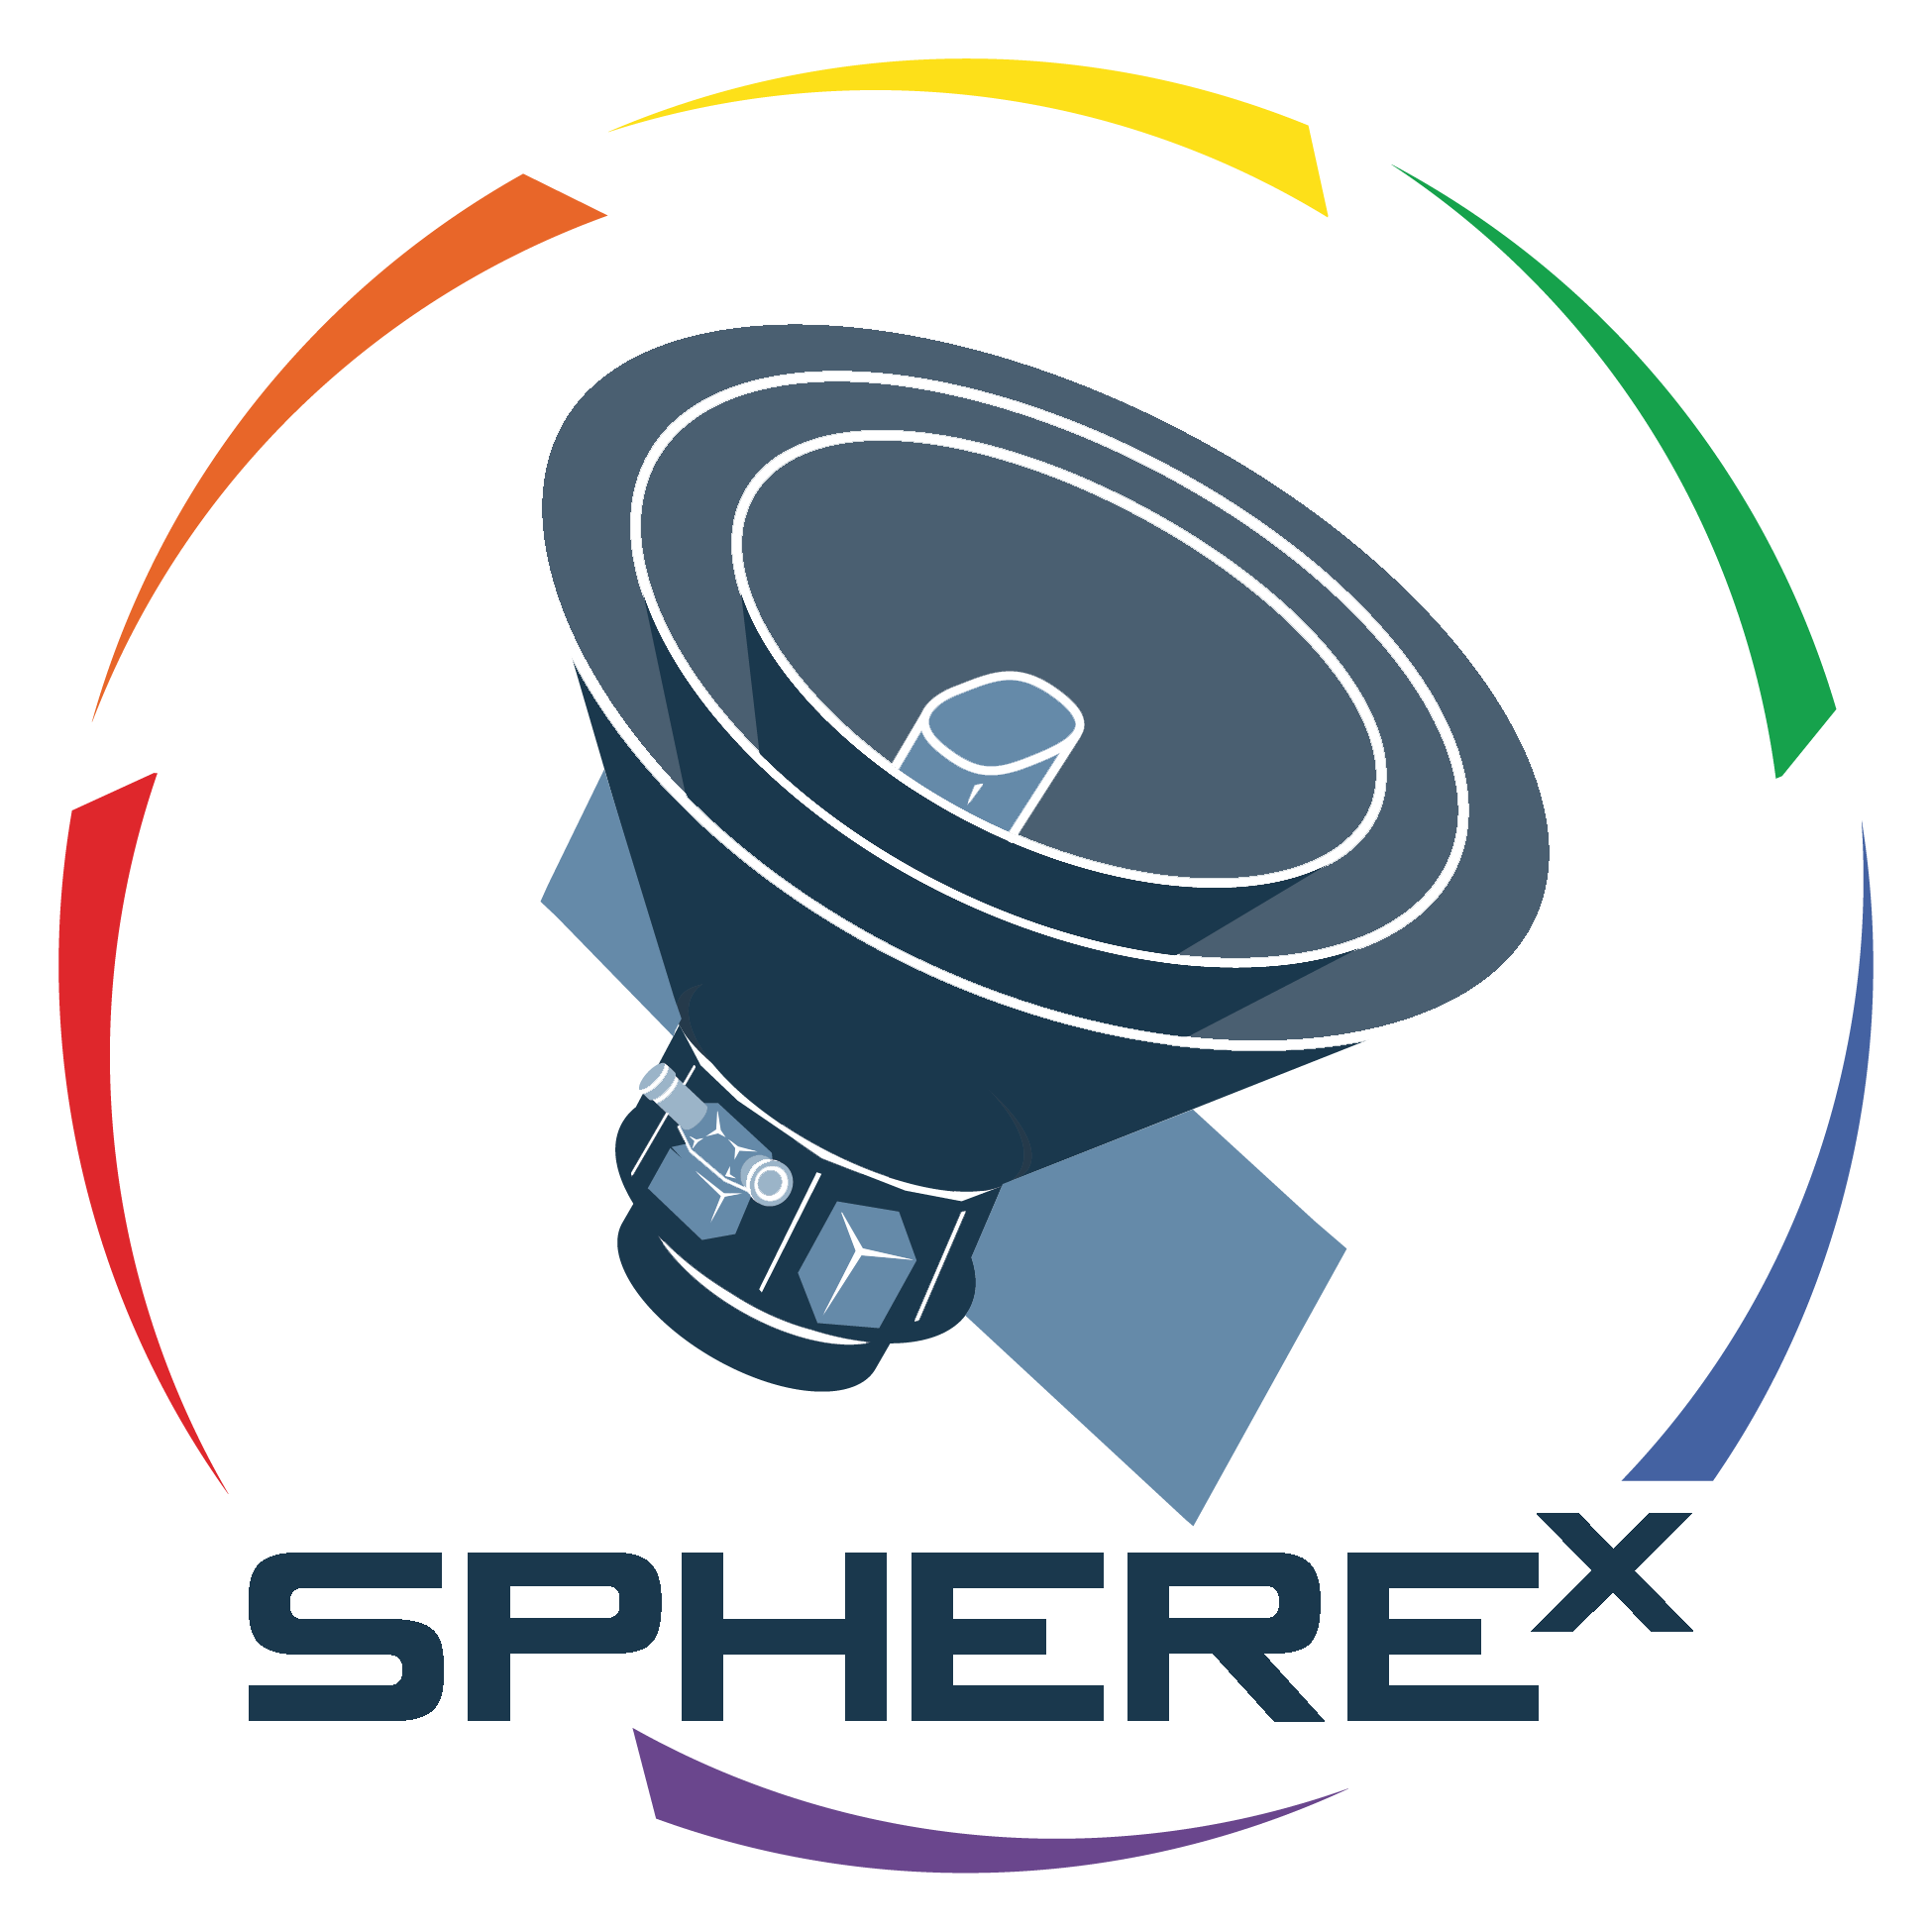
\includegraphics[height=0.5in]{./images/SPHEREx_logo.png}}
\chead{\large\spherex\ \vspace{1pt}{Test and Calibration Control and Archive Software: User Guide}}
\rhead{\version}
\footskip = 25pt
\cfoot{Page \thepage\ of \pageref{LastPage}}

\newcommand{\eps}{e$^{-}$ s$^{-1}$}

\newcommand{\spherex}{SPHEREx}

\begin{document}
	\begin{center}
		{\Large\bf SPHEREx Test and Calibration Control and Archive Software: User Guide}
		\vskip 0.25in
		{\large\bf \today} \\
		{\large\bf \version} \\
		\vskip 0.25in
		Sam Condon \texttt{scondon@caltech.edu} \\
		Marco Viero \texttt{mviero@caltech.edu} 
		\vskip 0.125in
	\end{center}
	
\section*{Introduction}

  The SPHEREx Test and Calibration Control and Archive Software provides a Python based toolset allowing a user to interface with the suite of SPHEREx spectral and focus calibration instrumentation. The toolset allows a user to manually control instruments in a measurement setup or specify fully automated measurement runs. This document provides a practical guide on how to use this toolset.

\tableofcontents


\section{Spectral Calibration Control}

This section details the control of the SPHEREx spectral calibration instrumentation. As of version \version, control of spectral calibration instrumentation can only be achieved using a GUI application, though a command-line interface is planned to be developed in future versions. In \version, the following instruments are integrated into the control interface:

\begin{enumerate}
\item Oriel/Newport CS260 Monochromator \\
\item Edmund Optics High-Speed Filter Wheel (referred to as NDF wheel) \\
\item Stanford Research Systems Sr510 and Sr830 Lockin Amplifiers \\
\item Labjack U6 (for warm shutter control) \\
\item Thorlabs S410C, S122C, and ajk;fdlsdlfsa;kjdjklfsa; detectors
\end{enumerate}

\subsection{GUI}
  Control of the spectral calibration instrumentation can be accomplished via a GUI. This section details how to use the GUI to run manual and automated measurements with the spectral calibration instrument suite.

\subsubsection{Startup}

  To launch the latest version of the spectral calibration GUI, navigate to the \emph{SPHEREx-Calibration-Automation} directory within the \emph{SPHEREx-Lab-Tools} repository and run the following command:

\begin{lstlisting}[language=bash]
python spherex_calibration.py spectral
\end{lstlisting}

Upon successful startup, a window similar to what is seen in figure (\ref{spectral cal gui}) will appear. Take note of the two main tabs provided by the interface, \emph{Automation} and \emph{Manual}. The purpose of each of these tabs is exactly as it sounds. \emph{Automation} can be used to create and run automated measurements while \emph{Manual} allows manual control and readout of the instruments present in the setup. The operation of each of these tabs is described in detail in the subsequent sections.

\begin{figure}[H]
\centering
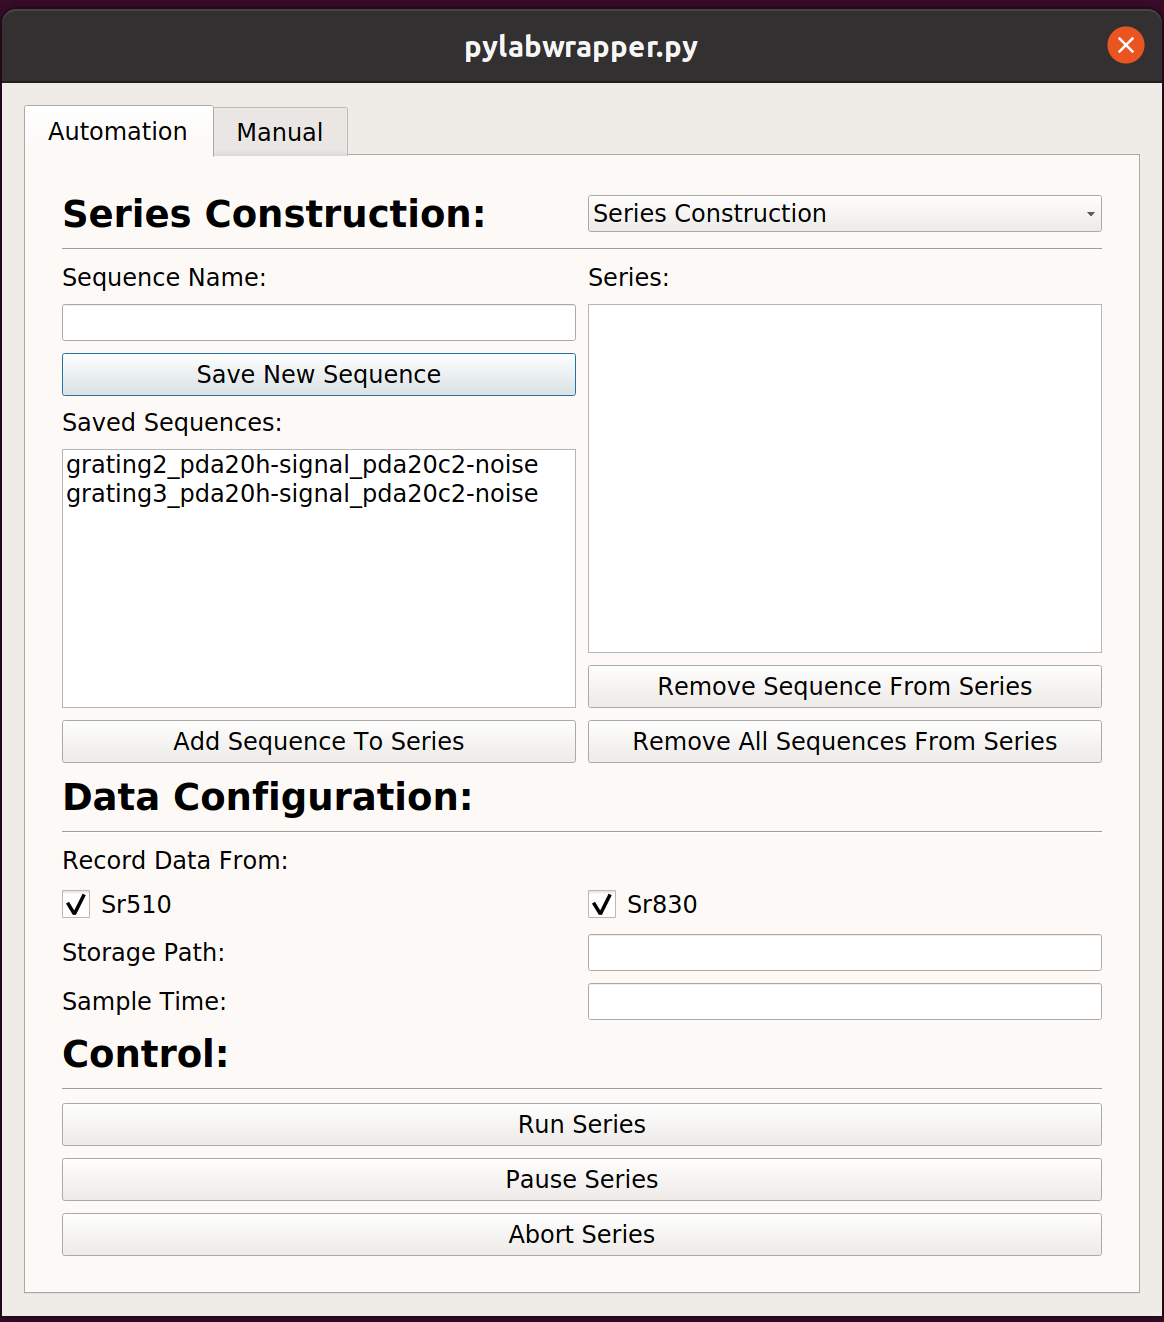
\includegraphics[width=0.5\linewidth]{./images/SpectralCalControlMainWindow.png}
\caption{Spectral Calibration Control Main Window}
\label{spectral cal gui}
\end{figure}

\subsubsection{Manual Tab}

The manual tab allows the user to manually control the instruments in the spectral calibration setup. As of version \version, the instruments that are integrated into the control include

\subsubsection{Automation Tab}
	
	
\end{document}